% figures/ioi_comparison.tex -- IOI Oracle Efficiency bar chart
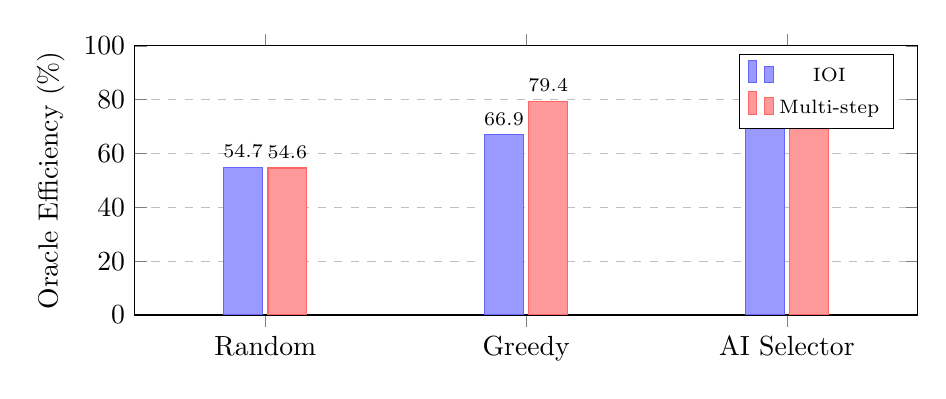
\begin{tikzpicture}
\begin{axis}[
    ybar,
    width=0.95\columnwidth,
    height=5cm,
    bar width=14pt,
    enlarge x limits=0.25,
    ylabel={Oracle Efficiency (\%)},
    symbolic x coords={Random, Greedy, AI Selector},
    xtick=data,
    ymin=0, ymax=100,
    ytick={0,20,40,60,80,100},
    nodes near coords,
    nodes near coords align={vertical},
    every node near coord/.append style={font=\scriptsize},
    legend style={at={(0.97,0.97)}, anchor=north east, font=\scriptsize},
    ymajorgrids=true,
    grid style=dashed,
]

% IOI task
\addplot[fill=blue!40, draw=blue!60] coordinates {
    (Random, 54.7) (Greedy, 66.9) (AI Selector, 74.4)
};

% Multi-step task
\addplot[fill=red!40, draw=red!60] coordinates {
    (Random, 54.6) (Greedy, 79.4) (AI Selector, 78.4)
};

\legend{IOI, Multi-step}
\end{axis}
\end{tikzpicture}
